% Options for packages loaded elsewhere
\PassOptionsToPackage{unicode}{hyperref}
\PassOptionsToPackage{hyphens}{url}
\PassOptionsToPackage{dvipsnames,svgnames,x11names}{xcolor}
%
\documentclass[
  letterpaper,
  DIV=11,
  numbers=noendperiod]{scrartcl}

\usepackage{amsmath,amssymb}
\usepackage{iftex}
\ifPDFTeX
  \usepackage[T1]{fontenc}
  \usepackage[utf8]{inputenc}
  \usepackage{textcomp} % provide euro and other symbols
\else % if luatex or xetex
  \usepackage{unicode-math}
  \defaultfontfeatures{Scale=MatchLowercase}
  \defaultfontfeatures[\rmfamily]{Ligatures=TeX,Scale=1}
\fi
\usepackage{lmodern}
\ifPDFTeX\else  
    % xetex/luatex font selection
\fi
% Use upquote if available, for straight quotes in verbatim environments
\IfFileExists{upquote.sty}{\usepackage{upquote}}{}
\IfFileExists{microtype.sty}{% use microtype if available
  \usepackage[]{microtype}
  \UseMicrotypeSet[protrusion]{basicmath} % disable protrusion for tt fonts
}{}
\makeatletter
\@ifundefined{KOMAClassName}{% if non-KOMA class
  \IfFileExists{parskip.sty}{%
    \usepackage{parskip}
  }{% else
    \setlength{\parindent}{0pt}
    \setlength{\parskip}{6pt plus 2pt minus 1pt}}
}{% if KOMA class
  \KOMAoptions{parskip=half}}
\makeatother
\usepackage{xcolor}
\setlength{\emergencystretch}{3em} % prevent overfull lines
\setcounter{secnumdepth}{-\maxdimen} % remove section numbering
% Make \paragraph and \subparagraph free-standing
\ifx\paragraph\undefined\else
  \let\oldparagraph\paragraph
  \renewcommand{\paragraph}[1]{\oldparagraph{#1}\mbox{}}
\fi
\ifx\subparagraph\undefined\else
  \let\oldsubparagraph\subparagraph
  \renewcommand{\subparagraph}[1]{\oldsubparagraph{#1}\mbox{}}
\fi

\usepackage{color}
\usepackage{fancyvrb}
\newcommand{\VerbBar}{|}
\newcommand{\VERB}{\Verb[commandchars=\\\{\}]}
\DefineVerbatimEnvironment{Highlighting}{Verbatim}{commandchars=\\\{\}}
% Add ',fontsize=\small' for more characters per line
\usepackage{framed}
\definecolor{shadecolor}{RGB}{241,243,245}
\newenvironment{Shaded}{\begin{snugshade}}{\end{snugshade}}
\newcommand{\AlertTok}[1]{\textcolor[rgb]{0.68,0.00,0.00}{#1}}
\newcommand{\AnnotationTok}[1]{\textcolor[rgb]{0.37,0.37,0.37}{#1}}
\newcommand{\AttributeTok}[1]{\textcolor[rgb]{0.40,0.45,0.13}{#1}}
\newcommand{\BaseNTok}[1]{\textcolor[rgb]{0.68,0.00,0.00}{#1}}
\newcommand{\BuiltInTok}[1]{\textcolor[rgb]{0.00,0.23,0.31}{#1}}
\newcommand{\CharTok}[1]{\textcolor[rgb]{0.13,0.47,0.30}{#1}}
\newcommand{\CommentTok}[1]{\textcolor[rgb]{0.37,0.37,0.37}{#1}}
\newcommand{\CommentVarTok}[1]{\textcolor[rgb]{0.37,0.37,0.37}{\textit{#1}}}
\newcommand{\ConstantTok}[1]{\textcolor[rgb]{0.56,0.35,0.01}{#1}}
\newcommand{\ControlFlowTok}[1]{\textcolor[rgb]{0.00,0.23,0.31}{#1}}
\newcommand{\DataTypeTok}[1]{\textcolor[rgb]{0.68,0.00,0.00}{#1}}
\newcommand{\DecValTok}[1]{\textcolor[rgb]{0.68,0.00,0.00}{#1}}
\newcommand{\DocumentationTok}[1]{\textcolor[rgb]{0.37,0.37,0.37}{\textit{#1}}}
\newcommand{\ErrorTok}[1]{\textcolor[rgb]{0.68,0.00,0.00}{#1}}
\newcommand{\ExtensionTok}[1]{\textcolor[rgb]{0.00,0.23,0.31}{#1}}
\newcommand{\FloatTok}[1]{\textcolor[rgb]{0.68,0.00,0.00}{#1}}
\newcommand{\FunctionTok}[1]{\textcolor[rgb]{0.28,0.35,0.67}{#1}}
\newcommand{\ImportTok}[1]{\textcolor[rgb]{0.00,0.46,0.62}{#1}}
\newcommand{\InformationTok}[1]{\textcolor[rgb]{0.37,0.37,0.37}{#1}}
\newcommand{\KeywordTok}[1]{\textcolor[rgb]{0.00,0.23,0.31}{#1}}
\newcommand{\NormalTok}[1]{\textcolor[rgb]{0.00,0.23,0.31}{#1}}
\newcommand{\OperatorTok}[1]{\textcolor[rgb]{0.37,0.37,0.37}{#1}}
\newcommand{\OtherTok}[1]{\textcolor[rgb]{0.00,0.23,0.31}{#1}}
\newcommand{\PreprocessorTok}[1]{\textcolor[rgb]{0.68,0.00,0.00}{#1}}
\newcommand{\RegionMarkerTok}[1]{\textcolor[rgb]{0.00,0.23,0.31}{#1}}
\newcommand{\SpecialCharTok}[1]{\textcolor[rgb]{0.37,0.37,0.37}{#1}}
\newcommand{\SpecialStringTok}[1]{\textcolor[rgb]{0.13,0.47,0.30}{#1}}
\newcommand{\StringTok}[1]{\textcolor[rgb]{0.13,0.47,0.30}{#1}}
\newcommand{\VariableTok}[1]{\textcolor[rgb]{0.07,0.07,0.07}{#1}}
\newcommand{\VerbatimStringTok}[1]{\textcolor[rgb]{0.13,0.47,0.30}{#1}}
\newcommand{\WarningTok}[1]{\textcolor[rgb]{0.37,0.37,0.37}{\textit{#1}}}

\providecommand{\tightlist}{%
  \setlength{\itemsep}{0pt}\setlength{\parskip}{0pt}}\usepackage{longtable,booktabs,array}
\usepackage{calc} % for calculating minipage widths
% Correct order of tables after \paragraph or \subparagraph
\usepackage{etoolbox}
\makeatletter
\patchcmd\longtable{\par}{\if@noskipsec\mbox{}\fi\par}{}{}
\makeatother
% Allow footnotes in longtable head/foot
\IfFileExists{footnotehyper.sty}{\usepackage{footnotehyper}}{\usepackage{footnote}}
\makesavenoteenv{longtable}
\usepackage{graphicx}
\makeatletter
\def\maxwidth{\ifdim\Gin@nat@width>\linewidth\linewidth\else\Gin@nat@width\fi}
\def\maxheight{\ifdim\Gin@nat@height>\textheight\textheight\else\Gin@nat@height\fi}
\makeatother
% Scale images if necessary, so that they will not overflow the page
% margins by default, and it is still possible to overwrite the defaults
% using explicit options in \includegraphics[width, height, ...]{}
\setkeys{Gin}{width=\maxwidth,height=\maxheight,keepaspectratio}
% Set default figure placement to htbp
\makeatletter
\def\fps@figure{htbp}
\makeatother
\newlength{\cslhangindent}
\setlength{\cslhangindent}{1.5em}
\newlength{\csllabelwidth}
\setlength{\csllabelwidth}{3em}
\newlength{\cslentryspacingunit} % times entry-spacing
\setlength{\cslentryspacingunit}{\parskip}
\newenvironment{CSLReferences}[2] % #1 hanging-ident, #2 entry spacing
 {% don't indent paragraphs
  \setlength{\parindent}{0pt}
  % turn on hanging indent if param 1 is 1
  \ifodd #1
  \let\oldpar\par
  \def\par{\hangindent=\cslhangindent\oldpar}
  \fi
  % set entry spacing
  \setlength{\parskip}{#2\cslentryspacingunit}
 }%
 {}
\usepackage{calc}
\newcommand{\CSLBlock}[1]{#1\hfill\break}
\newcommand{\CSLLeftMargin}[1]{\parbox[t]{\csllabelwidth}{#1}}
\newcommand{\CSLRightInline}[1]{\parbox[t]{\linewidth - \csllabelwidth}{#1}\break}
\newcommand{\CSLIndent}[1]{\hspace{\cslhangindent}#1}

<script type="text/x-mathjax-config">
MathJax.Hub.Config({
  TeX: { equationNumbers: {autoNumber: "AMS"} },
  tex2jax: {inlineMath: [ ['$','$'], ["\\(","\\)"] ]}
});
</script>

<!-- This is what works with Quarto -->
<script>
  MathJax = {
    tex: {
      tags: 'ams'  // should be 'ams', 'none', or 'all'
    }
  };
</script>
\usepackage{booktabs}
\usepackage{longtable}
\usepackage{array}
\usepackage{multirow}
\usepackage{wrapfig}
\usepackage{float}
\usepackage{colortbl}
\usepackage{pdflscape}
\usepackage{tabu}
\usepackage{threeparttable}
\usepackage{threeparttablex}
\usepackage[normalem]{ulem}
\usepackage{makecell}
\usepackage{xcolor}
\KOMAoption{captions}{tableheading}
\makeatletter
\@ifpackageloaded{tcolorbox}{}{\usepackage[skins,breakable]{tcolorbox}}
\@ifpackageloaded{fontawesome5}{}{\usepackage{fontawesome5}}
\definecolor{quarto-callout-color}{HTML}{909090}
\definecolor{quarto-callout-note-color}{HTML}{0758E5}
\definecolor{quarto-callout-important-color}{HTML}{CC1914}
\definecolor{quarto-callout-warning-color}{HTML}{EB9113}
\definecolor{quarto-callout-tip-color}{HTML}{00A047}
\definecolor{quarto-callout-caution-color}{HTML}{FC5300}
\definecolor{quarto-callout-color-frame}{HTML}{acacac}
\definecolor{quarto-callout-note-color-frame}{HTML}{4582ec}
\definecolor{quarto-callout-important-color-frame}{HTML}{d9534f}
\definecolor{quarto-callout-warning-color-frame}{HTML}{f0ad4e}
\definecolor{quarto-callout-tip-color-frame}{HTML}{02b875}
\definecolor{quarto-callout-caution-color-frame}{HTML}{fd7e14}
\makeatother
\makeatletter
\makeatother
\makeatletter
\makeatother
\makeatletter
\@ifpackageloaded{caption}{}{\usepackage{caption}}
\AtBeginDocument{%
\ifdefined\contentsname
  \renewcommand*\contentsname{Table of contents}
\else
  \newcommand\contentsname{Table of contents}
\fi
\ifdefined\listfigurename
  \renewcommand*\listfigurename{List of Figures}
\else
  \newcommand\listfigurename{List of Figures}
\fi
\ifdefined\listtablename
  \renewcommand*\listtablename{List of Tables}
\else
  \newcommand\listtablename{List of Tables}
\fi
\ifdefined\figurename
  \renewcommand*\figurename{Figure}
\else
  \newcommand\figurename{Figure}
\fi
\ifdefined\tablename
  \renewcommand*\tablename{Table}
\else
  \newcommand\tablename{Table}
\fi
}
\@ifpackageloaded{float}{}{\usepackage{float}}
\floatstyle{ruled}
\@ifundefined{c@chapter}{\newfloat{codelisting}{h}{lop}}{\newfloat{codelisting}{h}{lop}[chapter]}
\floatname{codelisting}{Listing}
\newcommand*\listoflistings{\listof{codelisting}{List of Listings}}
\makeatother
\makeatletter
\@ifpackageloaded{caption}{}{\usepackage{caption}}
\@ifpackageloaded{subcaption}{}{\usepackage{subcaption}}
\makeatother
\makeatletter
\@ifpackageloaded{tcolorbox}{}{\usepackage[skins,breakable]{tcolorbox}}
\makeatother
\makeatletter
\@ifundefined{shadecolor}{\definecolor{shadecolor}{rgb}{.97, .97, .97}}
\makeatother
\makeatletter
\makeatother
\makeatletter
\makeatother
\ifLuaTeX
  \usepackage{selnolig}  % disable illegal ligatures
\fi
\IfFileExists{bookmark.sty}{\usepackage{bookmark}}{\usepackage{hyperref}}
\IfFileExists{xurl.sty}{\usepackage{xurl}}{} % add URL line breaks if available
\urlstyle{same} % disable monospaced font for URLs
\hypersetup{
  pdftitle={Descriptive Statistics},
  pdfauthor={Daniela Palleschi},
  colorlinks=true,
  linkcolor={blue},
  filecolor={Maroon},
  citecolor={Blue},
  urlcolor={Blue},
  pdfcreator={LaTeX via pandoc}}

\title{Descriptive Statistics}
\usepackage{etoolbox}
\makeatletter
\providecommand{\subtitle}[1]{% add subtitle to \maketitle
  \apptocmd{\@title}{\par {\large #1 \par}}{}{}
}
\makeatother
\subtitle{Measures of central tendency and dispersion}
\author{Daniela Palleschi}
\date{Wed den 06.12.2023}

\begin{document}
\maketitle
\ifdefined\Shaded\renewenvironment{Shaded}{\begin{tcolorbox}[breakable, borderline west={3pt}{0pt}{shadecolor}, frame hidden, enhanced, sharp corners, boxrule=0pt, interior hidden]}{\end{tcolorbox}}\fi

\hypertarget{learning-objects}{%
\subsection*{Learning objects}\label{learning-objects}}
\addcontentsline{toc}{subsection}{Learning objects}

In this section we will learn\ldots{}

\begin{itemize}
\tightlist
\item
  about measures of central tendency (mean, median, mode)
\item
  about measures of dispersion (range, standard deviation)
\item
  how to use the \texttt{summarise()} function from \texttt{dplyr}
\item
  how to produce summaries \texttt{.by} group
\end{itemize}

\hypertarget{resources}{%
\subsection*{Resources}\label{resources}}
\addcontentsline{toc}{subsection}{Resources}

Some suggested readings for this topic are:

\begin{enumerate}
\def\labelenumi{\arabic{enumi}.}
\item
  Ch. 3, Sections 3.4-3.9 (\emph{Descriptive statistics, models, and
  distributions}) in @winter\_statistics\_2019 (available online for
  students/employees of the HU Berlin via the
  \href{https://hu-berlin.hosted.exlibrisgroup.com/permalink/f/uig076/TN_cdi_askewsholts_vlebooks_9781351677431}{HU
  Grimm Zentrum}.
\item
  \href{https://r4ds.hadley.nz/data-transform\#groups}{Section 4.5
  (Groups)} in Ch. 4 (\emph{Data Transformation}) in
  @wickham\_tidyverse\_2023.
\end{enumerate}

\hypertarget{set-up}{%
\subsection{Set-up}\label{set-up}}

\hypertarget{clear-environment}{%
\subsubsection{Clear Environment}\label{clear-environment}}

An important step we haven't talked about much yet is making sure you
\emph{always} start a new script with a clear R environment. This means
that we shouldn't have any objects stored in the Environment, but we
also shouldn't have any packages loaded. This is because we want to make
sure everything we are doing is achieved solely in this script, and is
not dependent on a package or data we had loaded from some other script.
To achieve this, you can click
\texttt{Session\ \textgreater{}\ Restart\ R} to start with a fresh
environment, or use the keyboard shortcut
\texttt{Cmd/Ctrl+Shift/Strg+0}.

\hypertarget{packages}{%
\subsubsection{Packages}\label{packages}}

We need to load the \texttt{tidyverse}, \texttt{here}, and
\texttt{janitor} packages. The latter two we need because we'll be
loading in local CSV datasets.

\begin{Shaded}
\begin{Highlighting}[]
\NormalTok{pacman}\SpecialCharTok{::}\FunctionTok{p\_load}\NormalTok{(tidyverse,}
\NormalTok{               here,}
\NormalTok{               janitor)}
\end{Highlighting}
\end{Shaded}

\hypertarget{load-data}{%
\subsubsection{Load data}\label{load-data}}

We will be using two datasets today: a slightly altered version of the
\texttt{groesse\_geburtstag} dataset from the last section
(\texttt{groesse\_geburtstag\_ws2324.csv}), and
\texttt{languageR\_english.csv}, which is a shorter version of the
\texttt{english} dataset from the \texttt{languageR} package. If you
don't have these data already, download them directly into your
\texttt{daten} folder from the course GitHub (press `Download raw file'
near the `Raw' button):

\begin{itemize}
\tightlist
\item
  \href{https://github.com/daniela-palleschi/r4ling_student/blob/main/daten/languageR_english.csv}{languageR\_english.csv}
\item
  \href{https://github.com/daniela-palleschi/r4ling_student/blob/main/daten/groesse_geburtstag_ws2324.csv}{groesse\_geburtstag\_ws2324.csv}
\end{itemize}

\begin{Shaded}
\begin{Highlighting}[]
\NormalTok{df\_groesse }\OtherTok{\textless{}{-}} \FunctionTok{read\_csv}\NormalTok{(}\FunctionTok{here}\NormalTok{(}\StringTok{"daten"}\NormalTok{, }\StringTok{"groesse\_geburtstag\_ws2324.csv"}\NormalTok{))}
\end{Highlighting}
\end{Shaded}

\begin{Shaded}
\begin{Highlighting}[]
\NormalTok{df\_eng }\OtherTok{\textless{}{-}} \FunctionTok{read\_csv}\NormalTok{(}\FunctionTok{here}\NormalTok{(}\StringTok{"daten"}\NormalTok{, }\StringTok{"languageR\_english.csv"}\NormalTok{)) }\SpecialCharTok{|\textgreater{}} 
  \FunctionTok{clean\_names}\NormalTok{() }\SpecialCharTok{|\textgreater{}} 
  \CommentTok{\# fix some wonky variable names:}
  \FunctionTok{rename}\NormalTok{(}\AttributeTok{rt\_lexdec =}\NormalTok{ r\_tlexdec,}
         \AttributeTok{rt\_naming =}\NormalTok{ r\_tnaming)}
\end{Highlighting}
\end{Shaded}

\hypertarget{deskriptive-statistics}{%
\subsection{Deskriptive statistics}\label{deskriptive-statistics}}

Descriptive statistics qunatitatively describe the central tendency,
variability, and distribution of data. They are sometimes also referred
to as summary statistics, because we \emph{summarise} the observed data.
Some common summary statistics include the range of values (minimum,
maximum), the mean value, and the standard deviation. Descriptive
statistics help us to the full scope understand our data, and are an
important step in exploring our dataset before running more advanced
\emph{inferential} statistics (which we will not cover in this course).

\hypertarget{number-of-observations-n}{%
\subsubsection{\texorpdfstring{Number of observations
(\(n\))}{Number of observations (n)}}\label{number-of-observations-n}}

The number of observations in a dataset is not a statistic, but is
important information when summarising or describing data. When we have
more data (higher \(n\)), we can have more confidence in the conclusions
we draw from our data because we have more evidence. Conversely, when we
have less data (lower \(n\)), our summary statistics may not be
generalisable to the broader population. We can check the number of
observations in a dataset using the native R \texttt{nrow()} function:

\begin{Shaded}
\begin{Highlighting}[]
\FunctionTok{nrow}\NormalTok{(df\_groesse)}
\end{Highlighting}
\end{Shaded}

\begin{verbatim}
[1] 9
\end{verbatim}

\begin{tcolorbox}[enhanced jigsaw, colframe=quarto-callout-note-color-frame, rightrule=.15mm, breakable, coltitle=black, opacityback=0, leftrule=.75mm, colback=white, toprule=.15mm, opacitybacktitle=0.6, colbacktitle=quarto-callout-note-color!10!white, bottomrule=.15mm, toptitle=1mm, left=2mm, titlerule=0mm, arc=.35mm, title=\textcolor{quarto-callout-note-color}{\faInfo}\hspace{0.5em}{\texttt{length()} versus \texttt{nrow()}}, bottomtitle=1mm]

The function \texttt{length()} tells us how many (horizontal) values
there are in an object. If that object is a data frame (instead of a
vector), it tells us how many \emph{columns} we have.

\begin{Shaded}
\begin{Highlighting}[]
\FunctionTok{length}\NormalTok{(df\_groesse)}
\end{Highlighting}
\end{Shaded}

\begin{verbatim}
[1] 5
\end{verbatim}

However, if that object is a vector, then \texttt{length()} gives us the
number of observations.

\begin{Shaded}
\begin{Highlighting}[]
\NormalTok{vector }\OtherTok{\textless{}{-}} \FunctionTok{c}\NormalTok{(}\DecValTok{1}\NormalTok{,}\DecValTok{5}\NormalTok{,}\DecValTok{2}\NormalTok{,}\DecValTok{6}\NormalTok{,}\DecValTok{8}\NormalTok{,}\DecValTok{4}\NormalTok{,}\DecValTok{7}\NormalTok{,}\DecValTok{8}\NormalTok{,}\DecValTok{3}\NormalTok{)}
\FunctionTok{length}\NormalTok{(vector)}
\end{Highlighting}
\end{Shaded}

\begin{verbatim}
[1] 9
\end{verbatim}

\end{tcolorbox}

\hypertarget{measures-of-central-tendency}{%
\subsubsection{Measures of central
tendency}\label{measures-of-central-tendency}}

Measures of central tendency quantitavely describe the centre of our
data. You have likely already encounted three measures of central
tendency before: the mean, median, and mode.

\hypertarget{mean-mu-or-barx}{%
\paragraph{\texorpdfstring{Mean (\(\mu\) or
\(\bar{x}\))}{Mean (\textbackslash mu or \textbackslash bar\{x\})}}\label{mean-mu-or-barx}}

The \texttt{mean}, or average, is the sum of all values divided by the
number of values (as in Equation \ref{eq-mean}). In mathematical
notation, \emph{sum} is written with the capital Greek sigma (\(\sum\)),
as in Equation \ref{eq-sigma}.

\begin{align}
\mu &= \frac{sum\;of\;values} 
           {n} \label{eq-mean} \\
\bar{x} &= \frac{\sum{x}}      
           {n} \label{eq-sigma} 
\end{align}

\hypertarget{population-mean-mu-versus-sample-mean-barx}{%
\paragraph{\texorpdfstring{Population mean (\(\mu\)) versus sample mean
(\(\bar{x}\))}{Population mean (\textbackslash mu) versus sample mean (\textbackslash bar\{x\})}}\label{population-mean-mu-versus-sample-mean-barx}}

Both equations mean the same thing, but use different notation to
represent the same equation. While \(\mu\) represents the
\emph{population mean}, while \(\bar{x}\) represents the \emph{sample
mean}. The population mean is the true mean of some measure in an entire
population (e.g., heights of all students at the Humboldt-Universität zu
Berlin). A \emph{sample} mean is the mean of a \emph{sample population}
from which we collected our data. For example, we have 9 observations in
\texttt{df\_groesse}. This data represents a sample of data from a
larger population.

\begin{center}\rule{0.5\linewidth}{0.5pt}\end{center}

We can easily compute the mean by hand when we have only a few values.
Recall our dataset from last week where we collected our heights in
centimeters
(\texttt{171,\ 168,\ 182,\ 190,\ 170,\ 163,\ 164,\ 167,\ 189}). There
are 9 values, so we have to add up these heights and divide the total by
9.

\begin{Shaded}
\begin{Highlighting}[]
\DecValTok{171}\SpecialCharTok{+} \DecValTok{168}\SpecialCharTok{+} \DecValTok{182}\SpecialCharTok{+} \DecValTok{190}\SpecialCharTok{+} \DecValTok{170}\SpecialCharTok{+} \DecValTok{163}\SpecialCharTok{+} \DecValTok{164}\SpecialCharTok{+} \DecValTok{167}\SpecialCharTok{+} \DecValTok{189} \SpecialCharTok{/} \DecValTok{9}
\end{Highlighting}
\end{Shaded}

\begin{verbatim}
[1] 1396
\end{verbatim}

This produces a mean height of 1396 cm. This can't be right, so what
went wrong? We can fix the equation above by wrapping the heights with
parantheses (\texttt{()}) before dividing by \(n\).

\begin{Shaded}
\begin{Highlighting}[]
\NormalTok{(}\DecValTok{171}\SpecialCharTok{+} \DecValTok{168}\SpecialCharTok{+} \DecValTok{182}\SpecialCharTok{+} \DecValTok{190}\SpecialCharTok{+} \DecValTok{170}\SpecialCharTok{+} \DecValTok{163}\SpecialCharTok{+} \DecValTok{164}\SpecialCharTok{+} \DecValTok{167}\SpecialCharTok{+} \DecValTok{189}\NormalTok{) }\SpecialCharTok{/} \DecValTok{9}
\end{Highlighting}
\end{Shaded}

\begin{verbatim}
[1] 173.7778
\end{verbatim}

This problem was caused by the \emph{order of operations}, which is
described in more detail below. The important thing to remember is that
you can be sure the \emph{outcome} of a certain operation will be
performed before any other operations if you wrap it in parantheses.

\begin{tcolorbox}[enhanced jigsaw, colframe=quarto-callout-tip-color-frame, rightrule=.15mm, breakable, coltitle=black, opacityback=0, leftrule=.75mm, colback=white, toprule=.15mm, opacitybacktitle=0.6, colbacktitle=quarto-callout-tip-color!10!white, bottomrule=.15mm, toptitle=1mm, left=2mm, titlerule=0mm, arc=.35mm, title=\textcolor{quarto-callout-tip-color}{\faLightbulb}\hspace{0.5em}{PEMDAS}, bottomtitle=1mm]

You might recall learning about the order of operations in math class as
a kid. This refers to the order of execution when we have a mathematical
equation with multiple operators, such as division, addition, and
multiplication. \texttt{R} follows \texttt{PEMDAS}, which stands for:

\begin{table}
\centering
\begin{tabular}{l|l|l}
\hline
letter & operation & R\\
\hline
P & parantheses & (x + y)\\
\hline
E & exponents & x\textasciicircum{}y\\
\hline
M & mutiply & x*y\\
\hline
D & divide & x/y\\
\hline
A & addition & x + y\\
\hline
S & subtraction & x - y\\
\hline
\end{tabular}
\end{table}

So, if an equation has more than one operation, such as
\texttt{171+\ 168+\ 182+\ 190+\ 170+\ 163+\ 164+\ 167+\ 189\ /\ 9},
which has both addition and division, the division will take place
first: \texttt{189\ /\ 9} occurs before addition all the numbers
together. This is why we wrap the addition of the observations in
parantheses to ensure we are dividing the \emph{sum} of these numbers by
\texttt{9}, rather than adding the first 8 numbers with the quotient of
\texttt{189\ /\ 9} (i.e., \texttt{21}).

\end{tcolorbox}

We can also save the results of an equation as an object, or multiple
values as a vector (a list of values of the same class). We could then
use the functions \texttt{sum()} and \texttt{length()} to compute the
mean, or simply use the \texttt{mean()} function.

\begin{Shaded}
\begin{Highlighting}[]
\CommentTok{\# save heights as a vector}
\NormalTok{heights }\OtherTok{\textless{}{-}} \FunctionTok{c}\NormalTok{(}\DecValTok{171}\NormalTok{, }\DecValTok{168}\NormalTok{, }\DecValTok{182}\NormalTok{, }\DecValTok{190}\NormalTok{, }\DecValTok{170}\NormalTok{, }\DecValTok{163}\NormalTok{, }\DecValTok{164}\NormalTok{, }\DecValTok{167}\NormalTok{, }\DecValTok{189}\NormalTok{)}
\CommentTok{\# divide the sum of heights by the n of heights}
\FunctionTok{sum}\NormalTok{(heights)}\SpecialCharTok{/}\FunctionTok{length}\NormalTok{(heights)}
\end{Highlighting}
\end{Shaded}

\begin{verbatim}
[1] 173.7778
\end{verbatim}

\begin{Shaded}
\begin{Highlighting}[]
\CommentTok{\# or use the mean() function}
\FunctionTok{mean}\NormalTok{(heights)}
\end{Highlighting}
\end{Shaded}

\begin{verbatim}
[1] 173.7778
\end{verbatim}

Our data is not often stored in a single vector, but rather a dataset.
We can run the \texttt{mean()} function on a variable in a data frame by
using the \texttt{\$} operator to indicate we want to select a column
from a data frame (\texttt{dataframe\$variable}).

\begin{Shaded}
\begin{Highlighting}[]
\FunctionTok{mean}\NormalTok{(df\_groesse}\SpecialCharTok{$}\NormalTok{groesse)}
\end{Highlighting}
\end{Shaded}

\begin{verbatim}
[1] 173.6667
\end{verbatim}

The \texttt{\$} operator is part of native R, and similar to
\texttt{df\_groesse\ \textbar{}\textgreater{}select(groesse)} in
\texttt{dplyr} syntax.

\hypertarget{median}{%
\paragraph{Median}\label{median}}

Another measure of central tendency is the \texttt{median}, which is the
the value in the middle of the dataset. If you line up all your values
in ascending (or descending) order, the middle value is the median. For
example, if you have 5 values, the 3rd value is the median. If you have
6 values, the mean of the 3rd and 4th values are the median. Half of the
data lie below the median, and half above it.

To sort our data in ascending order using base R, we can use the
\texttt{sort()} function. We can then just count which is the middle
value:

\begin{Shaded}
\begin{Highlighting}[]
\FunctionTok{sort}\NormalTok{(df\_groesse}\SpecialCharTok{$}\NormalTok{groesse)}
\end{Highlighting}
\end{Shaded}

\begin{verbatim}
[1] 163 164 167 167 170 171 182 189 190
\end{verbatim}

This is easy when we just have a few observations. We could
alternatively just use the function \texttt{median()}.

\begin{Shaded}
\begin{Highlighting}[]
\FunctionTok{median}\NormalTok{(df\_groesse}\SpecialCharTok{$}\NormalTok{groesse)}
\end{Highlighting}
\end{Shaded}

\begin{verbatim}
[1] 170
\end{verbatim}

An important feature of the median is that it is not affected by
outliers, or extreme values. Let's see what happens when we change our
tallest height (190cm) to be the height of the current tallest person in
the world: 251 cm.

\begin{Shaded}
\begin{Highlighting}[]
\NormalTok{df\_groesste }\OtherTok{\textless{}{-}}\NormalTok{ df\_groesse }\SpecialCharTok{|\textgreater{}} \FunctionTok{mutate}\NormalTok{(}\AttributeTok{groesse =} \FunctionTok{ifelse}\NormalTok{(groesse }\SpecialCharTok{==} \DecValTok{190}\NormalTok{, }\DecValTok{251}\NormalTok{, groesse))}
\end{Highlighting}
\end{Shaded}

\begin{Shaded}
\begin{Highlighting}[]
\FunctionTok{sort}\NormalTok{(df\_groesste}\SpecialCharTok{$}\NormalTok{groesse)}
\end{Highlighting}
\end{Shaded}

\begin{verbatim}
[1] 163 164 167 167 170 171 182 189 251
\end{verbatim}

\begin{Shaded}
\begin{Highlighting}[]
\FunctionTok{median}\NormalTok{(df\_groesste}\SpecialCharTok{$}\NormalTok{groesse)}
\end{Highlighting}
\end{Shaded}

\begin{verbatim}
[1] 170
\end{verbatim}

\begin{Shaded}
\begin{Highlighting}[]
\FunctionTok{mean}\NormalTok{(df\_groesste}\SpecialCharTok{$}\NormalTok{groesse)}
\end{Highlighting}
\end{Shaded}

\begin{verbatim}
[1] 180.4444
\end{verbatim}

We see that the mean changed from approximately 174cm to 180cm. The
median remained the same (170 cm), however, because the middle value is
independent of the other values in a dataset. For this reason the median
is often reported instead of the mean for data that has heavy skews to
more extreme values, such as when reporting incomes in a population.
Average incomes can be greatly skewed due to a small group of extremely
high-earners, and are not typically representative of the income of the
majority of citizens.

\hypertarget{mode}{%
\paragraph{Mode}\label{mode}}

The \texttt{mode} is the value that occurs the most in a data set, and
is another measure of central tendency. There's no R function to
determine the \texttt{mode}, but we've already seen some common ways to
visualise it: with a histogram or a density plot.

\begin{Shaded}
\begin{Highlighting}[]
\NormalTok{df\_groesse }\SpecialCharTok{|\textgreater{}}
  \FunctionTok{ggplot}\NormalTok{(}\FunctionTok{aes}\NormalTok{(}\AttributeTok{x =}\NormalTok{ groesse)) }\SpecialCharTok{+}
  \FunctionTok{geom\_histogram}\NormalTok{(}\AttributeTok{binwidth =}\NormalTok{ .}\DecValTok{5}\NormalTok{) }\SpecialCharTok{+}
  \FunctionTok{theme\_minimal}\NormalTok{() }
\end{Highlighting}
\end{Shaded}

\begin{figure}[H]

{\centering 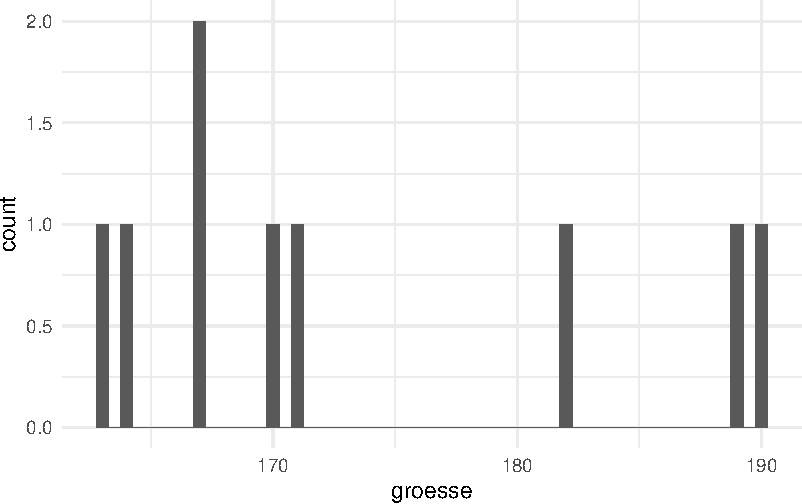
\includegraphics{08-desc_stats_en_files/figure-pdf/unnamed-chunk-22-1.pdf}

}

\end{figure}

\hypertarget{measures-of-dispersion}{%
\subsubsection{Measures of dispersion}\label{measures-of-dispersion}}

Measures of central tendency describe the middle of the data (usually).
Measures of dispersion describe the spread of data points, and tell us
something about how the data as a whole is distributed.

\hypertarget{range}{%
\paragraph{Range}\label{range}}

The \texttt{range} of values can refer to the highest (maximum) and
lowest (minimum) values, or the difference between highest and lowest
value.

\begin{center}\rule{0.5\linewidth}{0.5pt}\end{center}

The base R function \texttt{max()} and \texttt{min()} print the highest
and lowest values.

\begin{Shaded}
\begin{Highlighting}[]
\FunctionTok{max}\NormalTok{(heights)}
\end{Highlighting}
\end{Shaded}

\begin{verbatim}
[1] 190
\end{verbatim}

\begin{Shaded}
\begin{Highlighting}[]
\FunctionTok{min}\NormalTok{(heights)}
\end{Highlighting}
\end{Shaded}

\begin{verbatim}
[1] 163
\end{verbatim}

Or, we can simply use the \texttt{range()} function, which prints these
two numbers side-by-side.

\begin{Shaded}
\begin{Highlighting}[]
\FunctionTok{range}\NormalTok{(heights)}
\end{Highlighting}
\end{Shaded}

\begin{verbatim}
[1] 163 190
\end{verbatim}

We can find out the difference between these values by subtracting the
minimum value from the maximum value.

\begin{Shaded}
\begin{Highlighting}[]
\FunctionTok{max}\NormalTok{(heights) }\SpecialCharTok{{-}} \FunctionTok{min}\NormalTok{(heights)}
\end{Highlighting}
\end{Shaded}

\begin{verbatim}
[1] 27
\end{verbatim}

In a histogram or density plot, these values are represented by the
lowest and heights values on the x-axis.

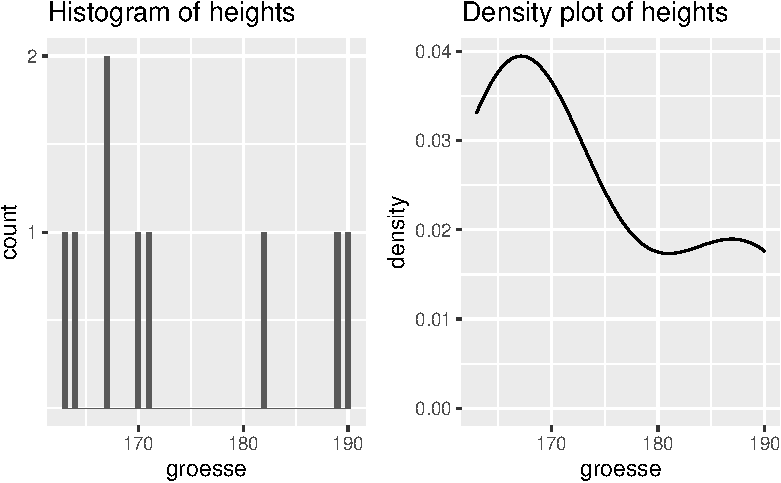
\includegraphics{08-desc_stats_en_files/figure-pdf/unnamed-chunk-27-1.pdf}

\hypertarget{standard-deviation-sd-or-sigma}{%
\paragraph{\texorpdfstring{Standard deviation (\texttt{sd} or
\(\sigma\))}{Standard deviation (sd or \textbackslash sigma)}}\label{standard-deviation-sd-or-sigma}}

Standard deviation is a measure of how dispersed data is \emph{in
relation to the mean}. A low standard deviation means data are clustered
around the mean (i.e., there is less spread), while a high standard
deviation means data are more spread out. Whether a standard deviation
is high or low is dependent on the scale and unit of measurement your
data is in. Standard deviation is very often given whenever mean is
reported.

Standard deviation (\texttt{sd}) is equal to the square root
(\(\sqrt{}\) or \texttt{sqrt()} in R) of the sum of squared value
deviations from the mean (\((x - \mu)^2\)) divided by the number of
observations minus 1 (\(n-1\)), given in Equation \ref{eq-sd}.

\begin{align}
\sigma & = \sqrt{\frac{(x_1-\mu)^2 + (x_2-\mu)^2 + ... + (x_N-\mu)^2}{N-1}} \label{eq-sd}
\end{align}

This looks intimidating, but we can calcuate standard deviation in R
using the \texttt{sd()} function.

\begin{Shaded}
\begin{Highlighting}[]
\FunctionTok{sd}\NormalTok{(heights)}
\end{Highlighting}
\end{Shaded}

\begin{verbatim}
[1] 10.46157
\end{verbatim}

However, knowing how to calculate standard deviation by hand gives us an
understanding of what the number represents. Let's practice calculating
standard deviation for a small set of values. Keeping in mind the
equation for standard deviation in \ref{eq-sd}, we can calculate
standard deviation by hand if we know the value of each observation, the
mean of these values, and the number of these values. For example, in a
vector with 3 observations (\texttt{3,5,9}), our values (\(x\)) are:

\begin{Shaded}
\begin{Highlighting}[]
\NormalTok{values }\OtherTok{\textless{}{-}} \FunctionTok{c}\NormalTok{(}\DecValTok{3}\NormalTok{,}\DecValTok{5}\NormalTok{,}\DecValTok{16}\NormalTok{)}
\NormalTok{values}
\end{Highlighting}
\end{Shaded}

\begin{verbatim}
[1]  3  5 16
\end{verbatim}

If we plug these into the equation for standard deviation we get
Equation \ref{eq-sd1}.

\begin{align}
\sigma & = \sqrt{\frac{(3-\mu)^2 + (5-\mu)^2 + (16-\mu)^2}{N-1}} \label{eq-sd1}
\end{align}

Our mean (\(\mu\)) is:

\begin{Shaded}
\begin{Highlighting}[]
\FunctionTok{mean}\NormalTok{(values)}
\end{Highlighting}
\end{Shaded}

\begin{verbatim}
[1] 8
\end{verbatim}

If we add this to Equation \ref{eq-sd1}, we get Equation \ref{eq-sd2}.

\begin{align}
\sigma & = \sqrt{\frac{(3-8)^2 + (5-8)^2 + (16-8)^2}{N-1}} \label{eq-sd2}
\end{align}

The number of values (\(n\)) is:

\begin{Shaded}
\begin{Highlighting}[]
\FunctionTok{length}\NormalTok{(values)}
\end{Highlighting}
\end{Shaded}

\begin{verbatim}
[1] 3
\end{verbatim}

If we add this to Equation \ref{eq-sd2}, we get Equation \ref{eq-sd3}.

\begin{align}
\sigma & = \sqrt{\frac{(3-8)^2 + (5-8)^2 + (16-8)^2}{3-1}} \label{eq-sd3}
\end{align}

If we carry out all of the operations following PEDMAS, then we get
Equations \ref{eq-sd4} through \ref{eq-sd}:

\begin{align}
\sigma & = \sqrt{\frac{(-5)^2 + (-3)^2 + (8)^2}{3-1}} \\ \label{eq-sd4}
\\
& = \sqrt{\frac{25 + 9 + 64}{3-1}}
\\
& = \sqrt{\frac{98}{2}} \\
& = \sqrt{49} \\
& = 7
\end{align}

To check our work, we calculate the standard deviation (\(\sigma\)) in
\texttt{R}:

\begin{Shaded}
\begin{Highlighting}[]
\FunctionTok{sd}\NormalTok{(values)}
\end{Highlighting}
\end{Shaded}

\begin{verbatim}
[1] 7
\end{verbatim}

\hypertarget{why-standard-deviation}{%
\subsubsection{Why standard deviation?}\label{why-standard-deviation}}

Standard deviation gives us a measure of how ``tight'' the observed
values are to the mean. If most of the observations are very close to
the mean, the standard deviation will be a small number relative to the
mean. If there are many observations with large deviations from the
mean, the standard deviation will tend to be a large number (relative to
the mean).

Different datasets can have the same mean but vastly different standard
deviations. For example:

\begin{Shaded}
\begin{Highlighting}[]
\NormalTok{values2 }\OtherTok{\textless{}{-}} \FunctionTok{c}\NormalTok{(}\DecValTok{55}\NormalTok{,}\DecValTok{55}\NormalTok{,}\DecValTok{55}\NormalTok{,}\DecValTok{55}\NormalTok{,}\DecValTok{55}\NormalTok{,}\DecValTok{57}\NormalTok{,}\DecValTok{57}\NormalTok{,}\DecValTok{57}\NormalTok{,}\DecValTok{57}\NormalTok{,}\DecValTok{57}\NormalTok{)}
\NormalTok{values3 }\OtherTok{\textless{}{-}} \FunctionTok{c}\NormalTok{(}\DecValTok{1}\NormalTok{,}\DecValTok{1}\NormalTok{,}\DecValTok{1}\NormalTok{,}\DecValTok{1}\NormalTok{,}\DecValTok{100}\NormalTok{,}\DecValTok{100}\NormalTok{,}\DecValTok{100}\NormalTok{,}\DecValTok{100}\NormalTok{,}\DecValTok{100}\NormalTok{)}
\end{Highlighting}
\end{Shaded}

\begin{Shaded}
\begin{Highlighting}[]
\FunctionTok{mean}\NormalTok{(values2)}
\end{Highlighting}
\end{Shaded}

\begin{verbatim}
[1] 56
\end{verbatim}

\begin{Shaded}
\begin{Highlighting}[]
\FunctionTok{mean}\NormalTok{(values3)}
\end{Highlighting}
\end{Shaded}

\begin{verbatim}
[1] 56
\end{verbatim}

We see that \texttt{values2} and \texttt{values3} have the same mean. We
might therefore conclude the data are similar. But their standard
deviations will differ, because their respective observed values all
differ in how far they deviate from the mean. Which vector do you think
will have the \emph{smallest} standard deviation? Why?

\begin{Shaded}
\begin{Highlighting}[]
\FunctionTok{sd}\NormalTok{(values2)}
\end{Highlighting}
\end{Shaded}

\begin{verbatim}
[1] 1.054093
\end{verbatim}

\begin{Shaded}
\begin{Highlighting}[]
\FunctionTok{sd}\NormalTok{(values3)}
\end{Highlighting}
\end{Shaded}

\begin{verbatim}
[1] 52.17758
\end{verbatim}

The larger standard deviation for \texttt{values3} reflects the fact
that the values tended to be very far from the mean. The smaller
standard deviation for \texttt{values2} reflects the fact that the value
for this variable tended to be quite close to the mean.

\begin{tcolorbox}[enhanced jigsaw, colframe=quarto-callout-note-color-frame, rightrule=.15mm, breakable, coltitle=black, opacityback=0, leftrule=.75mm, colback=white, toprule=.15mm, opacitybacktitle=0.6, colbacktitle=quarto-callout-note-color!10!white, bottomrule=.15mm, toptitle=1mm, left=2mm, titlerule=0mm, arc=.35mm, title=\textcolor{quarto-callout-note-color}{\faInfo}\hspace{0.5em}{Calculating standard deviation}, bottomtitle=1mm]

\begin{itemize}
\tightlist
\item
  first, calculate the deviation of each value from the mean

  \begin{itemize}
  \tightlist
  \item
    and square this value
  \end{itemize}
\item
  add up all these squared deviation values

  \begin{itemize}
  \tightlist
  \item
    divide by the number of observations \emph{minue one} (\(n-1\))
  \end{itemize}
\item
  this is now the \emph{variance}, to get the population standard
  deviation, compute the square root of this value
\end{itemize}

\begin{align}

\sigma & = \sqrt\frac{(171-173.8)^2 + (168-173.8)^2 + (182-173.8)^2 + (190-173.8)^2 + (170-173.8)^2 +
        (163-173.8)^2 + (164-173.8)^2 + (167-173.8)^2 + (189-173.8)^2 }{9-1}
\\
& = \sqrt\frac{(-2.8)^2 + (-5.8)^2 + (8.2)^2 + (16.2)^2 + (-3.8)^2 +
        (-10.8)^2 + (-9.8)^2 + (-6.8)^2 + (15.2)^2 }{9-1}
\\
& = \sqrt\frac{7.84 + 33.64 + 67.24 + 262.44 + 14.44 +
        116.64 + 96.04 + 46.24 + 231.04 }{9-1}
\\
& = \sqrt{\frac{875.56}{8}}
\\
& = \sqrt{109.445}
\\
& = 10.4616

\end{align}

Why do we square each observation's deviance from the mean, only to
later calculate the square root of their sum divided by \(N-1\)? Since
half of our observations will lie below the mean and half above, when we
subtract the mean from the values half of the resulting differences will
be negative and half of them positive. When we add positive and negative
values together, they cancel each other out. So, if we square all these
deviations from the mean, all the values will be positive (a positive
number multiplied by a positive number is a positive number, while a
negative number multiplied by itself also results in a positive number).
If we then calculate the square root of these values, we'd get the
original magnitude of the deviance but always as a positive value.

\end{tcolorbox}

\begin{tcolorbox}[enhanced jigsaw, colframe=quarto-callout-tip-color-frame, rightrule=.15mm, breakable, coltitle=black, opacityback=0, leftrule=.75mm, colback=white, toprule=.15mm, opacitybacktitle=0.6, colbacktitle=quarto-callout-tip-color!10!white, bottomrule=.15mm, toptitle=1mm, left=2mm, titlerule=0mm, arc=.35mm, title=\textcolor{quarto-callout-tip-color}{\faLightbulb}\hspace{0.5em}{Population properties}, bottomtitle=1mm]

Both the mean and standard deviation tell us something about the
population from which our data sample comes from. The more observations
we collect, the more precise these measures will tend to be on average.

\end{tcolorbox}

\hypertarget{summary-statistics-with-r}{%
\subsection{Summary statistics with R}\label{summary-statistics-with-r}}

We've already seen some useful functions to calculate summary statistics
(e.g., \texttt{mean()}, \texttt{median()}, \texttt{sd()}). However, we
will typically want to produce multiple summary statistics at once, and
to compare summary statistics between groups. To achieve this, the
\texttt{dplyr} package from the \texttt{tidyverse} has some helpful
functions. Let's now use the \texttt{df\_eng} dataset to learn about
these \texttt{dplyr} verbs.

\hypertarget{dplyrsummarise}{%
\subsubsection{\texorpdfstring{\texttt{dplyr::summarise}}{dplyr::summarise}}\label{dplyrsummarise}}

The \texttt{summarise()} function from \texttt{dplyr} computes summaries
of data, but we have to tell it \emph{what} to compute, and for which
variable(s). For example, the \texttt{n()} function produces the number
of observations (only when used inside \texttt{summarise()} or
\texttt{mutate()}). Let's first check how many observations we have in
the \texttt{df\_eng} dataset:

\begin{Shaded}
\begin{Highlighting}[]
\NormalTok{df\_eng }\SpecialCharTok{|\textgreater{}}
  \FunctionTok{summarise}\NormalTok{(}\AttributeTok{N =} \FunctionTok{n}\NormalTok{())}
\end{Highlighting}
\end{Shaded}

\begin{verbatim}
# A tibble: 1 x 1
      N
  <int>
1  4568
\end{verbatim}

Now let's take a look at a histogram of \texttt{rt\_lexdec}, the
variable containing lexical decision response times in milliseconds:

\begin{Shaded}
\begin{Highlighting}[]
\NormalTok{df\_eng }\SpecialCharTok{|\textgreater{}} 
  \FunctionTok{ggplot}\NormalTok{() }\SpecialCharTok{+}
  \FunctionTok{aes}\NormalTok{(}\AttributeTok{x =}\NormalTok{ rt\_lexdec) }\SpecialCharTok{+}
  \FunctionTok{geom\_histogram}\NormalTok{()}
\end{Highlighting}
\end{Shaded}

\begin{figure}[H]

{\centering 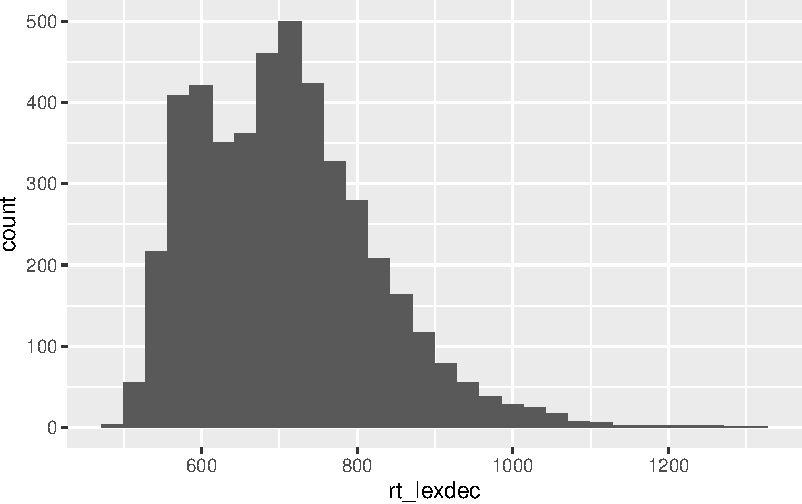
\includegraphics{08-desc_stats_en_files/figure-pdf/unnamed-chunk-39-1.pdf}

}

\end{figure}

We see that response time ranged from about 500 ms to 1320 ms, with most
responses between 550 ms and 900 ms. We also see a \emph{bimodal}
distribution, in that there are two modes (two peaks). The overall mode
is around 700 ms (500 observations), with a second peak around 600 ms
(\textasciitilde420 observations).

We can also run multiple computations at once. Let's also generate the
mean and standard deviation of the lexical decision task
(\texttt{rt\_lexdec}, in milliseconds).

\begin{Shaded}
\begin{Highlighting}[]
\NormalTok{df\_eng }\SpecialCharTok{|\textgreater{}}
  \FunctionTok{summarise}\NormalTok{(}\AttributeTok{mean\_lexdec =} \FunctionTok{mean}\NormalTok{(rt\_lexdec, }\AttributeTok{na.rm=}\NormalTok{T),}
            \AttributeTok{sd\_lexdec =} \FunctionTok{sd}\NormalTok{(rt\_lexdec, }\AttributeTok{na.rm =}\NormalTok{ T),}
            \AttributeTok{N =} \FunctionTok{n}\NormalTok{()) }
\end{Highlighting}
\end{Shaded}

\begin{verbatim}
# A tibble: 1 x 3
  mean_lexdec sd_lexdec     N
        <dbl>     <dbl> <int>
1        708.      115.  4568
\end{verbatim}

Now we see that the average lexical decision response time was 708.1 ms,
with a standard deviation of 114.9.

And we can specify calculations using typical mathematical operators
(e.g., \texttt{+,\ -,\ /,\ *,\ \^{}} \ldots) and/or functions. What was
the difference between the longest and the shortest lexical decision
response time?

\begin{Shaded}
\begin{Highlighting}[]
\NormalTok{df\_eng }\SpecialCharTok{|\textgreater{}}
  \FunctionTok{summarise}\NormalTok{(}\AttributeTok{range\_lexdec =} \FunctionTok{max}\NormalTok{(rt\_lexdec) }\SpecialCharTok{{-}} \FunctionTok{min}\NormalTok{(rt\_lexdec))}
\end{Highlighting}
\end{Shaded}

\begin{verbatim}
# A tibble: 1 x 1
  range_lexdec
         <dbl>
1         828.
\end{verbatim}

\begin{tcolorbox}[enhanced jigsaw, colframe=quarto-callout-tip-color-frame, rightrule=.15mm, breakable, coltitle=black, opacityback=0, leftrule=.75mm, colback=white, toprule=.15mm, opacitybacktitle=0.6, colbacktitle=quarto-callout-tip-color!10!white, bottomrule=.15mm, toptitle=1mm, left=2mm, titlerule=0mm, arc=.35mm, title=\textcolor{quarto-callout-tip-color}{\faLightbulb}\hspace{0.5em}{Missing values}, bottomtitle=1mm]

Some calculations aren't possible if there are missing values. The
variable \texttt{rt\_naming} has a missing value. We can see that in the
output from the \texttt{summary()} function, which removes any
\texttt{NA} values before computing summary statistics.

\begin{Shaded}
\begin{Highlighting}[]
\NormalTok{df\_eng }\SpecialCharTok{|\textgreater{}}
  \FunctionTok{select}\NormalTok{(rt\_lexdec, rt\_naming) }\SpecialCharTok{|\textgreater{}}
  \FunctionTok{summary}\NormalTok{()}
\end{Highlighting}
\end{Shaded}

\begin{verbatim}
   rt_lexdec        rt_naming    
 Min.   : 495.4   Min.   :412.3  
 1st Qu.: 617.4   1st Qu.:468.1  
 Median : 699.6   Median :570.6  
 Mean   : 708.1   Mean   :565.9  
 3rd Qu.: 775.3   3rd Qu.:658.4  
 Max.   :1323.2   Max.   :808.9  
                  NA's   :1      
\end{verbatim}

The \texttt{mean()} function does \emph{not} remove \texttt{NA} values,
however.

\begin{Shaded}
\begin{Highlighting}[]
\NormalTok{df\_eng }\SpecialCharTok{|\textgreater{}}
  \FunctionTok{summarise}\NormalTok{(}\AttributeTok{mean\_naming =} \FunctionTok{mean}\NormalTok{(rt\_naming))}
\end{Highlighting}
\end{Shaded}

\begin{verbatim}
# A tibble: 1 x 1
  mean_naming
        <dbl>
1          NA
\end{verbatim}

What do we do with missing values? When working with real data, how we
deal with missing values is not trivial. E.g., we might want to convert
all \texttt{NA} values to \texttt{0} if we want them to contribute to
the calculation of the \texttt{mean}. More often than not though we want
to just remove them.

We can easily do this with the \texttt{dplyr} verb \texttt{drop\_na()}:

\begin{Shaded}
\begin{Highlighting}[]
\NormalTok{df\_eng }\SpecialCharTok{|\textgreater{}}
  \FunctionTok{drop\_na}\NormalTok{() }\SpecialCharTok{|\textgreater{}}
  \FunctionTok{summarise}\NormalTok{(}\AttributeTok{mean\_naming =} \FunctionTok{mean}\NormalTok{(rt\_naming))}
\end{Highlighting}
\end{Shaded}

\begin{verbatim}
# A tibble: 1 x 1
  mean_naming
        <dbl>
1        566.
\end{verbatim}

\end{tcolorbox}

\hypertarget{grouping-variables}{%
\subsection{Grouping variables}\label{grouping-variables}}

We don't always just want to know the summary statistics for an entire
dataset, however. We usually want to \emph{compare} certain groups
(e.g., comparing \texttt{groesse} between L1 speaker groups)

\hypertarget{by}{%
\subsubsection{\texorpdfstring{\texttt{.by\ =}}{.by =}}\label{by}}

The brand new (and experimental) \texttt{.by\ =} argument in
\texttt{summarise()} computes our calculations on grouped subsets of the
data. It takes a \texttt{variable} (i.e., column name), and groups by
the levels of this variable.

\begin{center}\rule{0.5\linewidth}{0.5pt}\end{center}

\begin{Shaded}
\begin{Highlighting}[]
\NormalTok{df\_eng }\SpecialCharTok{|\textgreater{}}
  \FunctionTok{drop\_na}\NormalTok{() }\SpecialCharTok{|\textgreater{}}
  \FunctionTok{summarise}\NormalTok{(}\AttributeTok{mean\_lexdec =} \FunctionTok{mean}\NormalTok{(rt\_lexdec),}
            \AttributeTok{sd\_lexdec =} \FunctionTok{sd}\NormalTok{(rt\_lexdec),}
            \AttributeTok{N =} \FunctionTok{n}\NormalTok{(),}
            \AttributeTok{.by =}\NormalTok{ age\_subject) }\SpecialCharTok{|\textgreater{}}
  \FunctionTok{arrange}\NormalTok{(mean\_lexdec)}
\end{Highlighting}
\end{Shaded}

\begin{verbatim}
# A tibble: 2 x 4
  age_subject mean_lexdec sd_lexdec     N
  <chr>             <dbl>     <dbl> <int>
1 young              630.      69.1  2283
2 old                787.      96.2  2284
\end{verbatim}

\hypertarget{group-by-multiple-variables}{%
\subsubsection{Group by multiple
variables}\label{group-by-multiple-variables}}

\begin{itemize}
\tightlist
\item
  we can also group by multiple variables

  \begin{itemize}
  \tightlist
  \item
    for this we need \texttt{concatenate} (\texttt{c()})
  \end{itemize}
\item
  we'll filter to only have a couple of carriers, just so our output
  isn't too long
\end{itemize}

\begin{center}\rule{0.5\linewidth}{0.5pt}\end{center}

\begin{Shaded}
\begin{Highlighting}[numbers=left,,]
\NormalTok{df\_eng }\SpecialCharTok{|\textgreater{}}
  \FunctionTok{drop\_na}\NormalTok{() }\SpecialCharTok{|\textgreater{}}
  \FunctionTok{summarise}\NormalTok{(}\AttributeTok{mean\_lexdec =} \FunctionTok{mean}\NormalTok{(rt\_lexdec),}
            \AttributeTok{sd\_lexdec =} \FunctionTok{sd}\NormalTok{(rt\_lexdec),}
            \AttributeTok{N =} \FunctionTok{n}\NormalTok{(),}
            \AttributeTok{.by =} \FunctionTok{c}\NormalTok{(age\_subject, word\_category)) }\SpecialCharTok{|\textgreater{}}
  \FunctionTok{arrange}\NormalTok{(age\_subject)}
\end{Highlighting}
\end{Shaded}

\begin{verbatim}
# A tibble: 4 x 5
  age_subject word_category mean_lexdec sd_lexdec     N
  <chr>       <chr>               <dbl>     <dbl> <int>
1 old         N                    790.     101.   1452
2 old         V                    780.      86.5   832
3 young       N                    633.      70.8  1451
4 young       V                    623.      65.7   832
\end{verbatim}

\begin{center}\rule{0.5\linewidth}{0.5pt}\end{center}

\begin{tcolorbox}[enhanced jigsaw, colframe=quarto-callout-note-color-frame, rightrule=.15mm, breakable, coltitle=black, opacityback=0, leftrule=.75mm, colback=white, toprule=.15mm, opacitybacktitle=0.6, colbacktitle=quarto-callout-note-color!10!white, bottomrule=.15mm, toptitle=1mm, left=2mm, titlerule=0mm, arc=.35mm, title=\textcolor{quarto-callout-note-color}{\faInfo}\hspace{0.5em}{\texttt{group\_by()}}, bottomtitle=1mm]

\begin{itemize}
\tightlist
\item
  before \texttt{.by()}, we used to use the \texttt{dplyr} verb
  \texttt{group\_by()} and \texttt{ungroup()}

  \begin{itemize}
  \tightlist
  \item
    I prefer the new \texttt{.by}, because it keeps the grouping local
    (no need to \texttt{ungroup()})
  \item
    keep this in mind, you might see \texttt{group\_by()} in the wild
  \end{itemize}
\end{itemize}

\begin{Shaded}
\begin{Highlighting}[numbers=left,,]
\NormalTok{df\_eng }\SpecialCharTok{|\textgreater{}}
  \FunctionTok{group\_by}\NormalTok{(age\_subject, word\_category) }\SpecialCharTok{|\textgreater{}} 
  \FunctionTok{summarise}\NormalTok{(}\AttributeTok{mean\_lexdec =} \FunctionTok{mean}\NormalTok{(rt\_lexdec),}
            \AttributeTok{sd\_lexdec =} \FunctionTok{sd}\NormalTok{(rt\_lexdec),}
            \AttributeTok{N =} \FunctionTok{n}\NormalTok{()) }\SpecialCharTok{|\textgreater{}} 
  \FunctionTok{ungroup}\NormalTok{() }\SpecialCharTok{|\textgreater{}} 
  \FunctionTok{arrange}\NormalTok{(age\_subject)}
\end{Highlighting}
\end{Shaded}

\begin{verbatim}
# A tibble: 4 x 5
  age_subject word_category mean_lexdec sd_lexdec     N
  <chr>       <chr>               <dbl>     <dbl> <int>
1 old         N                    790.     101.   1452
2 old         V                    780.      86.5   832
3 young       N                    633.      70.8  1452
4 young       V                    623.      65.7   832
\end{verbatim}

\end{tcolorbox}

\hypertarget{anscombes-quartet}{%
\subsection{Anscombe's Quartet}\label{anscombes-quartet}}

Francis Anscombe constructed 4 datasets in 1973 to illustrate the
importance of visualising data before analysing it and building a model.
These four plots represent 4 datasets that all have nearly identical
mean and standard deviation, but very different distributions.

\hypertarget{tbl-anscombe}{}
\begin{table}
\caption{\label{tbl-anscombe}Summary stats of Anscombe's quratet datasets }\tabularnewline

\centering\begingroup\fontsize{20}{22}\selectfont

\begin{tabular}{l|r|r|r|r|r|r|r}
\hline
grp & mean\_x & mean\_y & min\_x & min\_y & max\_x & max\_y & crrltn\\
\hline
Group 1 & 9 & 7.500909 & 4 & 4.26 & 14 & 10.84 & 0.8164205\\
\hline
Group 2 & 9 & 7.500909 & 4 & 3.10 & 14 & 9.26 & 0.8162365\\
\hline
Group 3 & 9 & 7.500000 & 4 & 5.39 & 14 & 12.74 & 0.8162867\\
\hline
Group 4 & 9 & 7.500909 & 8 & 5.25 & 19 & 12.50 & 0.8165214\\
\hline
\end{tabular}
\endgroup{}
\end{table}

\begin{center}\rule{0.5\linewidth}{0.5pt}\end{center}

\begin{figure}

{\centering 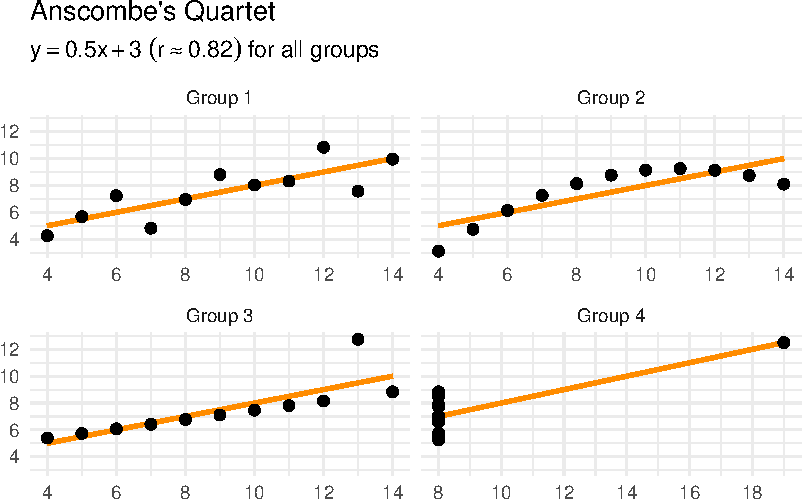
\includegraphics{08-desc_stats_en_files/figure-pdf/fig-anscombe-1.pdf}

}

\caption{\label{fig-anscombe}Plots of Anscombe's quratet distributions}

\end{figure}

\hypertarget{datasaurrus}{%
\subsubsection{DatasaurRus}\label{datasaurrus}}

The datasauRus package {[}@datasauRus-package{]} contains some more
datasets that have similar \texttt{mean} and \texttt{sd}, but different
distributions, given in Table~\ref{tbl-datasauRus}.

\begin{Shaded}
\begin{Highlighting}[]
\NormalTok{pacman}\SpecialCharTok{::}\FunctionTok{p\_load}\NormalTok{(}\StringTok{"datasauRus"}\NormalTok{)}
\end{Highlighting}
\end{Shaded}

\begin{Shaded}
\begin{Highlighting}[]
\NormalTok{datasaurus\_dozen }\SpecialCharTok{|\textgreater{}}
    \FunctionTok{group\_by}\NormalTok{(dataset) }\SpecialCharTok{|\textgreater{}}
    \FunctionTok{summarize}\NormalTok{(}
      \AttributeTok{mean\_x    =} \FunctionTok{mean}\NormalTok{(x),}
      \AttributeTok{mean\_y    =} \FunctionTok{mean}\NormalTok{(y),}
      \AttributeTok{std\_dev\_x =} \FunctionTok{sd}\NormalTok{(x),}
      \AttributeTok{std\_dev\_y =} \FunctionTok{sd}\NormalTok{(y),}
      \AttributeTok{corr\_x\_y  =} \FunctionTok{cor}\NormalTok{(x, y)}
\NormalTok{    ) }\SpecialCharTok{|\textgreater{}}
\NormalTok{  knitr}\SpecialCharTok{::}\FunctionTok{kable}\NormalTok{() }\SpecialCharTok{|\textgreater{}}
\NormalTok{  kableExtra}\SpecialCharTok{::}\FunctionTok{kable\_styling}\NormalTok{(}\AttributeTok{font\_size =} \DecValTok{20}\NormalTok{)}
\end{Highlighting}
\end{Shaded}

\hypertarget{tbl-datasauRus}{}
\begin{table}
\caption{\label{tbl-datasauRus}Summary stats of datasauRus datasets }\tabularnewline

\centering\begingroup\fontsize{20}{22}\selectfont

\begin{tabular}{l|r|r|r|r|r}
\hline
dataset & mean\_x & mean\_y & std\_dev\_x & std\_dev\_y & corr\_x\_y\\
\hline
away & 54.26610 & 47.83472 & 16.76983 & 26.93974 & -0.0641284\\
\hline
bullseye & 54.26873 & 47.83082 & 16.76924 & 26.93573 & -0.0685864\\
\hline
circle & 54.26732 & 47.83772 & 16.76001 & 26.93004 & -0.0683434\\
\hline
dino & 54.26327 & 47.83225 & 16.76514 & 26.93540 & -0.0644719\\
\hline
dots & 54.26030 & 47.83983 & 16.76774 & 26.93019 & -0.0603414\\
\hline
h\_lines & 54.26144 & 47.83025 & 16.76590 & 26.93988 & -0.0617148\\
\hline
high\_lines & 54.26881 & 47.83545 & 16.76670 & 26.94000 & -0.0685042\\
\hline
slant\_down & 54.26785 & 47.83590 & 16.76676 & 26.93610 & -0.0689797\\
\hline
slant\_up & 54.26588 & 47.83150 & 16.76885 & 26.93861 & -0.0686092\\
\hline
star & 54.26734 & 47.83955 & 16.76896 & 26.93027 & -0.0629611\\
\hline
v\_lines & 54.26993 & 47.83699 & 16.76996 & 26.93768 & -0.0694456\\
\hline
wide\_lines & 54.26692 & 47.83160 & 16.77000 & 26.93790 & -0.0665752\\
\hline
x\_shape & 54.26015 & 47.83972 & 16.76996 & 26.93000 & -0.0655833\\
\hline
\end{tabular}
\endgroup{}
\end{table}

If we plot the datasets, they all look very different
(Figure~\ref{fig-datasauRus})!

\begin{figure}

{\centering 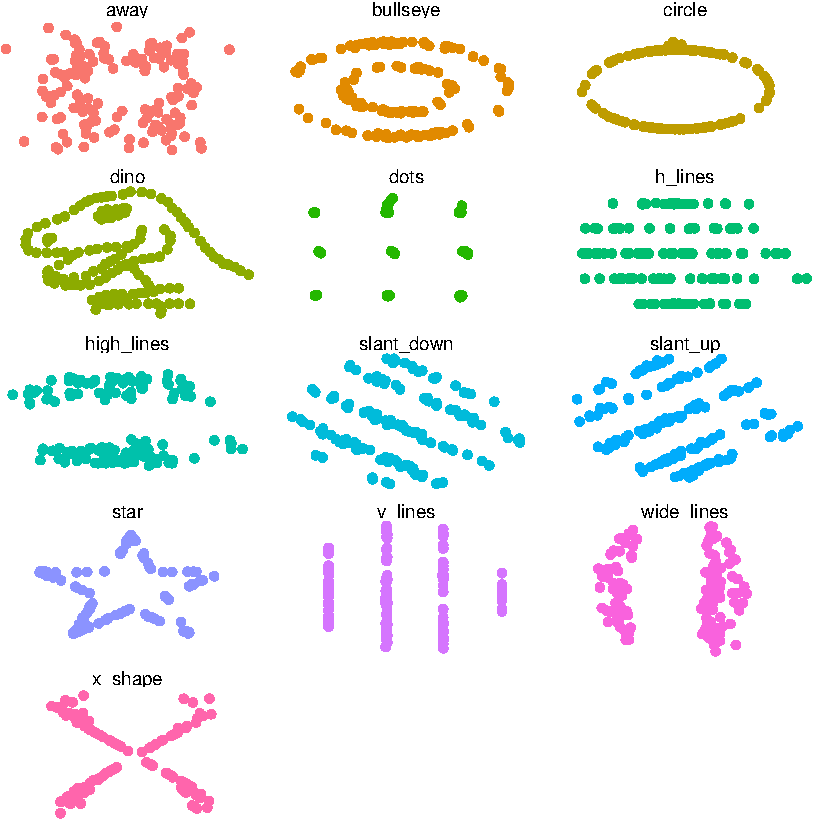
\includegraphics[width=0.5\textwidth,height=\textheight]{08-desc_stats_en_files/figure-pdf/fig-datasauRus-1.pdf}

}

\caption{\label{fig-datasauRus}Plots of datasauRus dataset
distributions}

\end{figure}

\begin{center}\rule{0.5\linewidth}{0.5pt}\end{center}

The point here being: \textbf{\emph{always plot your data}}, don't just
look at the descriptive stats!! Both are very important to understanding
your data. We've already seen how to plot our raw data using histograms,
density plots, barplots, and scatterplots. Next week we're going to look
at how to plot our summary statistics, and how to include the raw data
in the plot with multi-part plots.

\hypertarget{learning-objectives}{%
\subsection*{Learning objectives 🏁}\label{learning-objectives}}

Today we learned\ldots{}

\begin{itemize}
\tightlist
\item
  about measures of central tendency ✅
\item
  about measures of dispersion ✅
\item
  how to use the \texttt{summarise()} function from \texttt{dplyr} ✅
\item
  how to produce summaries \texttt{.by} group ✅
\end{itemize}

\hypertarget{aufgaben}{%
\subsection{Aufgaben}\label{aufgaben}}

\begin{enumerate}
\def\labelenumi{\arabic{enumi}.}
\tightlist
\item
  Calculate the standard deviation of the values
  \texttt{152,\ 19,\ 1398,\ 67,\ 2111} without using the function
  \texttt{sd()}

  \begin{itemize}
  \tightlist
  \item
    show your work. The following R syntax might be useful (depending on
    how you decide to do it):

    \begin{itemize}
    \tightlist
    \item
      \texttt{c()}
    \item
      \texttt{mean()}
    \item
      \texttt{x\^{}2} calculates the square of a value (here,
      \texttt{x})
    \item
      \texttt{sqrt()} calculates the square root
    \item
      \texttt{length()} produces the number of observations in a vector
    \end{itemize}
  \end{itemize}
\end{enumerate}

\begin{center}\rule{0.5\linewidth}{0.5pt}\end{center}

\begin{enumerate}
\def\labelenumi{\arabic{enumi}.}
\setcounter{enumi}{1}
\tightlist
\item
  Use the function \texttt{sd()} to print the standard deviation of the
  values above. Did you get it right?
\item
  Using \texttt{summarise}, print the mean, standard deviation, and
  number of observations for \texttt{dep\_delay}.

  \begin{itemize}
  \tightlist
  \item
    Hint: do you need to remove missing values (\texttt{NA}s)?
  \end{itemize}
\item
  Do the same, but add the \texttt{.by()} argument to find the departure
  delay (\texttt{dep\_delay}) per month

  \begin{itemize}
  \tightlist
  \item
    \texttt{arrange()} the output by the mean departure delay
  \end{itemize}
\end{enumerate}

\hypertarget{session-info}{%
\subsection*{Session Info}\label{session-info}}
\addcontentsline{toc}{subsection}{Session Info}

Created with R version 4.3.0 (2023-04-21) (Already Tomorrow) and
RStudioversion 2023.9.0.463 (Desert Sunflower).

\begin{Shaded}
\begin{Highlighting}[]
\FunctionTok{sessionInfo}\NormalTok{()}
\end{Highlighting}
\end{Shaded}

\begin{verbatim}
R version 4.3.0 (2023-04-21)
Platform: aarch64-apple-darwin20 (64-bit)
Running under: macOS Ventura 13.2.1

Matrix products: default
BLAS:   /Library/Frameworks/R.framework/Versions/4.3-arm64/Resources/lib/libRblas.0.dylib 
LAPACK: /Library/Frameworks/R.framework/Versions/4.3-arm64/Resources/lib/libRlapack.dylib;  LAPACK version 3.11.0

locale:
[1] en_US.UTF-8/en_US.UTF-8/en_US.UTF-8/C/en_US.UTF-8/en_US.UTF-8

time zone: Europe/Berlin
tzcode source: internal

attached base packages:
[1] stats     graphics  grDevices utils     datasets  methods   base     

other attached packages:
 [1] datasauRus_0.1.6 patchwork_1.1.3  janitor_2.2.0    here_1.0.1      
 [5] lubridate_1.9.2  forcats_1.0.0    stringr_1.5.0    dplyr_1.1.3     
 [9] purrr_1.0.2      readr_2.1.4      tidyr_1.3.0      tibble_3.2.1    
[13] ggplot2_3.4.3    tidyverse_2.0.0 

loaded via a namespace (and not attached):
 [1] gtable_0.3.4      xfun_0.39         lattice_0.21-8    tzdb_0.4.0       
 [5] vctrs_0.6.3       tools_4.3.0       generics_0.1.3    parallel_4.3.0   
 [9] fansi_1.0.4       pacman_0.5.1      pkgconfig_2.0.3   Matrix_1.5-4     
[13] webshot_0.5.4     lifecycle_1.0.3   compiler_4.3.0    farver_2.1.1     
[17] munsell_0.5.0     snakecase_0.11.0  htmltools_0.5.5   yaml_2.3.7       
[21] pillar_1.9.0      crayon_1.5.2      nlme_3.1-162      tidyselect_1.2.0 
[25] rvest_1.0.3       digest_0.6.33     stringi_1.7.12    labeling_0.4.3   
[29] splines_4.3.0     rprojroot_2.0.3   fastmap_1.1.1     grid_4.3.0       
[33] colorspace_2.1-0  cli_3.6.1         magrittr_2.0.3    utf8_1.2.3       
[37] withr_2.5.0       scales_1.2.1      bit64_4.0.5       timechange_0.2.0 
[41] rmarkdown_2.22    httr_1.4.6        bit_4.0.5         hms_1.1.3        
[45] kableExtra_1.3.4  evaluate_0.21     knitr_1.44        viridisLite_0.4.2
[49] mgcv_1.8-42       rlang_1.1.1       glue_1.6.2        xml2_1.3.4       
[53] svglite_2.1.1     rstudioapi_0.14   vroom_1.6.3       jsonlite_1.8.7   
[57] R6_2.5.1          systemfonts_1.0.4
\end{verbatim}

\hypertarget{literaturverzeichnis}{%
\subsection*{Literaturverzeichnis}\label{literaturverzeichnis}}

\hypertarget{refs}{}
\begin{CSLReferences}{0}{0}
\end{CSLReferences}



\end{document}
